\section{Problem definition : In-core fuel management optimization}

\subsection{PWR operation, in-core physics}

\noindent Nuclear reactor physics is a large field, however even if the main physics and models would be described by nuclear physics, neutronics (mainly neutron transport theory), in practice we can get a workaround based on expressions of the reactor by defining a few measurable parameters characterizing the reactor. Let us expose the usual configuration of a PWR reactor and the basic physics inside, then the main parameters used in the industry to discuss the reactor properties. 

\subsection{Problem definition and scope}
What is asked is to elaborate a list of artificial intelligence strategies allowing engineers to find faster a first almost-optimized loading pattern based on the optimization of the safety constraints, economical constraints and physical requirements. Let's evaluate a few of the variables (this is not an exhaustive list, just a reminder and variables that had been insisted on for in-core fuel management) : 

\begin{itemize}
\item \textbf{$k_{\infty}$ : } The multiplication factor of the reactor, that is the ratio of the fresh neutron population per fission cycle. Defined by the four-factor equation : $k_{\infty} = \eta \epsilon pf$. This grandeur allows us to evaluate if the chain-reaction can be sustained by the fuel. 

\item \textbf{FDH : }  Nuclear Enthalpy Rise Hot Channel Factor $(F^{N}_{\Delta H}$, this parameter is essential in PWR control as it gives a good insurance the core is far (or close) from a DNB scenario, in practice at Engie it has to be below 1.4 when using the assembling tools. \cite{DBN}

\begin{comment}
\item \textbf{FZ :}
\end{comment}
\item \textbf{Neutron poisons :} During operation, the part of $^{235}U$ atoms that undergo fission will create various fission products with different neutron absorption cross-sections, yield and decay rates. The huge absorption cross-section of $^{135}Xe$ in the thermal energy range makes it a great source of anti-reactivity and has to be taken into account. We distinguish two type of poisons, the ones creating \textbf{slagging}, which determines the natural life of the loading pattern (essential when planning a cycle). And nuclear \textbf{poisoning}, which diminishes global $k_{eff}$. Often we use neutron poisons to reduce the reactivity of fresh assemblies with $^{155}Gd$ and $^{157}Gd$ the two Gadolinium isotopes. It is thus used as a burnable absorber \cite{gado}. 
\item \textbf{Natural life : }Expected time (in MWd/tU) for the core to burn at full power until neutron poisons brings down the reactivity. After that time one can stretch up the fuel consumption for around thirty days at lower power to match the refueling schedule.
\item \textbf{MTC : } The moderator temperature coefficient, defined as the change in reactivity per degree change in the moderator temperature, mostly a function of the moderator-to-fuel ratio \cite{MTC}, when designing most safety guidelines order that \textit{“The MTC should be non-positive over the entire fuel cycle when the reactor is at a significant power level.”} (for LWR or PWR)

\item \textbf{Fluence : } We define the neutron fluence as the time integral of the neutron flux density. Not a quantifiable parameter for the reactor, but has to be taken into account in the LP design. It is expressed as number of particles $/cm^2$. It is important as it can be used as a measure of fuel burnup. It is also important to protect the structure of the reactor as it is a measure of the potency of the neutron flux of neutron embrittlement \cite{fluence}.

\item \textbf{Burnup and burnup gradient : } The burnup is defined as the measure of how much energy is being extracted from the fuel, and is used as a measure of fuel depletion \cite{burnup}. Essential to monitor has it is an essential part in the power distribution problem, power tilts (asymmetrical power distribution in the core), which imposes symmetry in the placing of assemblies in the LP-design. 
\end{itemize}

\noindent From the internal documentation at Engie, we define In-core fuel management as : 
\textit{calculating core reactivity, power distribution and isotropic inventory in order to meet these technical and economical requirements during subsequent cycles} \cite{engie19}. \\

\noindent We define on the other hand the loading pattern design as : \textit{find a suitable configuration of fresh and irradiated FA (= fuel assemblies) in order to meet the needs put forward by in-core fuel management}. \\

\noindent The tools used in house are \textbf{PANTHER}, \textbf{PANACHE}, \textbf{AUTUNITE} (Engie-developped) and \textbf{LPO} (Loading pattern optimizer). PANTHER is the 3D diffusion code for transient and steady-state core calculation. LPO gives an initial LP for the engineer to optimize further with the graphical interface of PANACHE, which presents itself as follow :

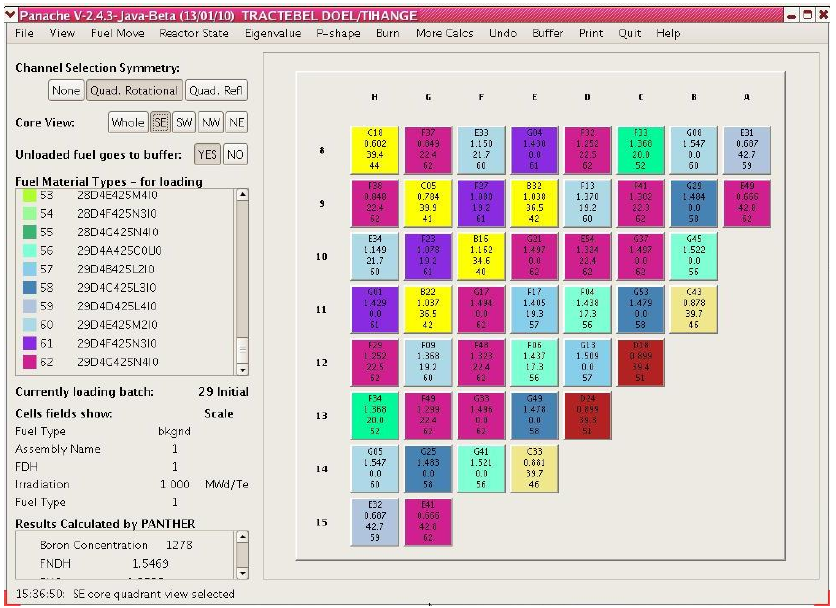
\includegraphics[scale = 0.6]{Figures/panther.png} \\

\noindent AUTUNITE searches the database if there is in the past design patterns that matches (or closely match) the constraint at the moment and propose a first LP based on the plan-required natural life and available fuel stocks in pools. The search query being faster than the LPO process. \\

\noindent The work is usually done by visualizing one quarter of the core, the reactor demanding a 8-axis symmetry this representation is sufficient. The user shuffles the cells until the design is satisfactory. A color scheme represents each cell reactivity and is given a name for identification in the fuel inventory. Furthermore is given all useful metrics for the whole core in the box on the left. 


\section{Machine learning tools in fuel management}

\noindent The \textit{Introduction to loading pattern design} gives a good idea of what type of input/output we are looking for. It is quite clear that the considering of all parameters would be out of scope for this project. Let's define : 

\subsection{Problem characterization}
\cite{ephraim19}, we see that the pseudo-code has to work as following : 
\begin{lstlisting}
INPUT :
    Stock assemblies
        Each assembly caracterized : 
            Burnup
            k_inf
            gadolinium content 
            enrichment 
            past position 

OUTPUT :
    Number of fresh assembly required 
    Loading pattern 
    (Risk and flexibility analysis)
    Gain evaluation 
\end{lstlisting}


\noindent The first approach (prototyping the propositions of the next paragraph) should only focus on the most important parameters of a loading pattern, that is the FDH, total reactivity and burnup tu match the given loading plan. For PWR the most critical security issue is the \textit{Departure From Nucleate Boiling} \cite{DBN} (DNB), that is when a local vapor layer forms around the core. When it happens, good heat transfer is not sufficient anymore and an huge amount of heat is accumulated at the core.






